
\documentclass[12pt,a4paper]{article}

% Türkçe %
\usepackage[utf8]{inputenc} %Türkçe karakterler için
\usepackage[T1]{fontenc}
\renewcommand{\tablename}{Tablo}
\renewcommand{\figurename}{Şekil}
\renewcommand{\indexname}{Dizin}
\renewcommand{\listfigurename}{Şekiller}
\renewcommand{\listtablename}{Tablolar}
\renewcommand{\contentsname}{İçindekiler}
\renewcommand{\refname}{Kaynaklar}
% Türkçe %

\usepackage{pdfpages}
\usepackage{geometry}
\usepackage{graphicx} %Resim koymak için
\usepackage{times} %Times fontu
\usepackage[nottoc]{tocbibind}
\usepackage{url}

\setcounter{tocdepth}{4}
\setcounter{secnumdepth}{4}

\newcommand{\subsubsubsection}[1]{\paragraph{#1}\mbox{}\\}

\begin{document}

    \pagenumbering{gobble}
    \begin{titlepage}
   \begin{center}
      \begin{large}
         \vspace*{0.5cm}
         GAZİ ÜNİVERSİTESİ \\
         MÜHENDİSLİK FAKÜLTESİ \\
         BİLGİSAYAR MÜHENDİSLİĞİ

         \vfill
         BM495  BİLGİSAYAR PROJESİ \\
         SPMP BELGESİ

         \vfill
         Abdullah Akalın\\Karim El Guermai\\Muhammed Emre Emrah\\

         \vfill
         \vspace{0.5cm}
         01.11.2017
      \end{large}
   \end{center}
\end{titlepage}

    \newpage

    \pagenumbering{roman}
    \tableofcontents
    \newpage

    \pagenumbering{arabic}

    \section{Genel Bakış}
    \subsection{Kapsam}
    Bu belgenin amacı grubumuzun üzerinde çalıştığı yapay öğrenme projesinin tasarım sürecini
    ele almak, takip edilen yaklaşımları açıklamak ve beklentileri değerlendirmektir. 

    \subsection{Amaç}
    Bu tasarım belgesi, projenin yapısal modelini belirtir, projenin hayata
    geçirilmesi için göz önüne alınacak tasarım unsurlarını açıklar ve gerekli
    görülen yerlerde bu unsurların birbirleriyle olan ilişkisini gösterir.

    \subsection{Hedef Kitlesi}
    Belgenin hedef kitlesi, projenin geliştiricileri, gözetmeni ve bu projeyle
    ilgilenen herkestir. 

    \section{Tanımlar}
    \textbf{Jupyter Notebook:} İçinde düz yazıların, kodların ve kod çıktılarının, hatta grafiklerin ve
    görsellerin bir arada bulunabildiği açık kaynaklı bir web uygulamasıdır. \cite{jupy}

    \section{Veri Bilimi Projelerinde Tasarım Sürecine Dair}
    Grubumuzun geliştirmeyi hedeflediği proje, bir veri bilimi araştırma projesidir.
    Veri bilimi usülleri, yazılım geliştirme usüllerinden biraz farklı bulunmaktadır.
    Zira yazılım geliştirme sürecinin sonucu bir bilgisayar kodudur, öte yandan
    bir veri bilimi projesi sonuç olarak bir konu hakkında çeşitli faydalı
    bilgilere vakıf olunmasını sağlar. 

    Veri bilimi, yazılım mühendisliğine nispetle yeni bir alandır. Bu durumun
    doğal bir sonucu olarak bu alanda proje geliştirmenin gelenekleşmiş bir
    yolu henüz tam olarak bulunmamaktadır. Aynı zamanda bir veri bilimi
    projesinde, projenin nasıl bir çıktı üreteceğinin önceden bilinmesi
    olanak dışıdır. 
    
    Bu nedenlerle yazılım mühendisliğine dayalı belgelendirmenin bir
    numunesi olan bu belgenin, veri bilimine has yukarıda bahsi geçen
    durumlar göz önüne alınarak değerlendirilmesi rica olunur.\cite{byrne}

    \section{Tasarım Bilgi İçeriği}
    \subsection{Belgenin Organizasyonu}
    İlk bölümde belgeye genel bakış yapılmıştır. Belgenin kapsam, amaç ve 
    hedef kitlesi belirtilmiştir. Daha sonra bu belgenin hazırlanmasında
    etkili olan kriterlere değinilmiştir. Ardından projenin tasarımında izlenen
    yollar açıklanıp belge sonuçlandırılmıştır.

    \subsection{Projenin Beklentileri}
    Bu projenin beklentisi, bir konu hakkında bir problemin, yapay öğrenme
    yöntemleriyle çözülmesiyle, o konuya dair çıkarımlarda bulunulmasıdır.
    Her ne kadar proje başlangıcında görüntü verilerine dair bir problem
    çözümü düşünülmüş olsa da, proje danışmanının yönlendirmesiyle sağlık alanında
    bit problem incelenmektedir.

    \subsection{Tasarım Katmanları}
    Söz konusu bir veri bilimi araştırma projesi olduğu için,
    klasik yazılım projelerine has veritabanı, önyüz, sunucu vb. katmanlar
    projemizde bulunmamaktadır. Ancak problemin tespiti, verinin elde edilmesi
    , analizi ve modellenmesi aşamaları ayrı katmanlar olarak düşünülebilir.
    Bu adımlar \ref{tasa} numaralı bölümde ayrıntılı olarak ele alınmıştır.

    \subsection{Tasarım Gerekçeleri}
    Projenin tekrar kullanılabilmesi ve değerlendirilebilmesi, atılan tüm
    adımların kaydedilmesine bağlıdır. Veri üzerinde yapılan tüm değişiklikler,
    öznitelik çıkarımları, veri üzerinde uygulanan fonksiyonlar aynı sırada
    ve aynı koşullar altında uygulanmalıdır. Bu yüzden projenin tasarım
    aşamalarında \textit{Jupyter Notebook} kullanılmıştır.

    \section{Proje Tasarımında İzlenen Yollar} \label{tasa}
    Projenin tasarımında \textit{"Harvard data science"} dersinde kullanılan
    aşamalar esas alınmıştır (bkz. \figurename{} \ref{flow}). Bu aşamalar müteakip bölümlerde
    açıklanmıştır. Belirtilmesi gereken bir husus şudur ki, bu aşamalar sadece
    yukarıdan aşağı ilerlemeyip, gerektiğinde aşağıdan yukarı geçişlere müsaade
    etmektedir.
    \begin{figure}
        \begin{center}
            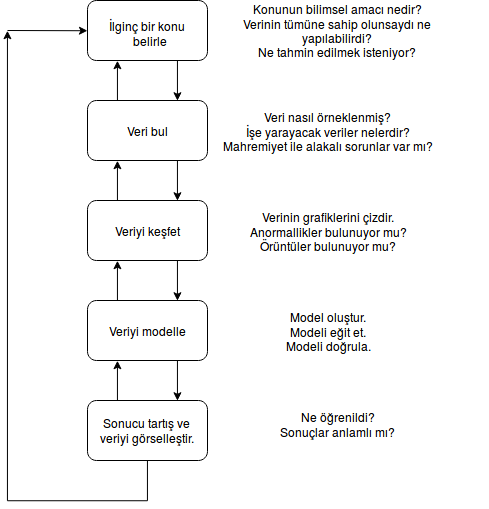
\includegraphics[width=\linewidth]{resimler/flow.png}
            \caption{Projede tasarımında kullanılan aşamalar. (\cite{byrne} kaynağından uyarlanmıştır.)}
            \label{flow}
        \end{center}
    \end{figure}

    \subsection{İlginç Bir Konunun Belirlenmesi}
    Bu aşama, projenin ana gayesini belirleyen aşamadır. 
    Belirlenen konuya dair bilgi edinilmesi de gerekebilmekte olup
    başarı kriterleri de yine konuyu bilenler ile birlikte değerlendirilmelidir.

    \subsection{Verinin Temin Edilmesi}
    Bu projede veri tarafımıza danışmanımızca sağlanmıştır. Ancak hazır verinin
    bulunmadığı taktirde verinin ölçümler sonucunda elde edilmesi gerekmektedir.

    \subsection{Verinin Keşfedilmesi}
    Bu aşama, eldeki verinin didiklenmesidir. Bu aşamada grafikler ve görseller
    kullanılarak verinin mahiyeti gözleme alınır. Bir sonraki aşama için gerekli
    altyapının oluşmasını sağlar.

    \subsection{Verinin Modellenmesi}
    İrdelenen veri, uygun görülen yöntemler kullanılarak modellenir. Hiçbir zaman
    bir model en iyisi değildir, bu yüzden birden çok modelin oluşturulması
    muhtemeldir. Modellerin sonuçları bir sonraki aşamaya aktarılır.

    \subsection{Sonucun Tartışılması ve Görselleştirilmesi}
    Modellerin sonuçları, belirlenen başarı kriterlerine göre belirlenir.
    Bir konuda, başarı gösteremeyen bir model,  üstün başarı gösteren
    bir modelin ifade ettiğinden daha az değere sahip değildir. Burada ölçüt
    hedeflenen ve ulaşılmak istenen bilgi ve kavrayıştır.

    \section{Sonuç}
    Bu belgede yapılmakta olan projenin tasarım aşamalarına ve unsurlarına yer verilmiştir.
    Veri bilimi projelerinin doğası gereği şimdi göz önünde bulundurulan bir hususun
    önemsiz olduğunun daha sonra anlaşılması yahut tam tersi durumların ortaya çıkması
    muhtemel olduğundan genel bir çerçeve çizilmeye çalışılmıştır. Nihai sonuç ancak
    proje tamamlandıktan sonra anlaşılabilecektir.

    \newpage
    \bibliography{kaynakca/kaynakca}
    \bibliographystyle{ieeetr}

\end{document}


